\documentclass{extbook}[14pt]
\usepackage{multicol, enumerate, enumitem, hyperref, color, soul, setspace, parskip, fancyhdr, amssymb, amsthm, amsmath, bbm, latexsym, units, mathtools}
\everymath{\displaystyle}
\usepackage[headsep=0.5cm,headheight=0cm, left=1 in,right= 1 in,top= 1 in,bottom= 1 in]{geometry}
\usepackage{dashrule}  % Package to use the command below to create lines between items
\newcommand{\litem}[1]{\item #1

\rule{\textwidth}{0.4pt}}
\pagestyle{fancy}
\lhead{}
\chead{Answer Key for Progress Quiz 5 Version C}
\rhead{}
\lfoot{9912-2038}
\cfoot{}
\rfoot{Spring 2021}
\begin{document}
\textbf{This key should allow you to understand why you choose the option you did (beyond just getting a question right or wrong). \href{https://xronos.clas.ufl.edu/mac1105spring2020/courseDescriptionAndMisc/Exams/LearningFromResults}{More instructions on how to use this key can be found here}.}

\textbf{If you have a suggestion to make the keys better, \href{https://forms.gle/CZkbZmPbC9XALEE88}{please fill out the short survey here}.}

\textit{Note: This key is auto-generated and may contain issues and/or errors. The keys are reviewed after each exam to ensure grading is done accurately. If there are issues (like duplicate options), they are noted in the offline gradebook. The keys are a work-in-progress to give students as many resources to improve as possible.}

\rule{\textwidth}{0.4pt}

\begin{enumerate}\litem{
Determine the domain of the function below.
\[ f(x) = \frac{6}{15x^{2} +27 x + 12} \]The solution is \( \text{All Real numbers except } x = -1.000 \text{ and } x = -0.800. \), which is option A.\begin{enumerate}[label=\Alph*.]
\item \( \text{All Real numbers except } x = a \text{ and } x = b, \text{ where } a \in [-1.16, -0.98] \text{ and } b \in [-0.99, -0.75] \)

All Real numbers except $x = -1.000$ and $x = -0.800$, which is the correct option.
\item \( \text{All Real numbers except } x = a, \text{ where } a \in [-20.05, -19.94] \)

All Real numbers except $x = -20.000$, which corresponds to removing a distractor value from the denominator.
\item \( \text{All Real numbers.} \)

This corresponds to thinking the denominator has complex roots or that rational functions have a domain of all Real numbers.
\item \( \text{All Real numbers except } x = a, \text{ where } a \in [-1.16, -0.98] \)

All Real numbers except $x = -1.000$, which corresponds to removing only 1 value from the denominator.
\item \( \text{All Real numbers except } x = a \text{ and } x = b, \text{ where } a \in [-20.05, -19.94] \text{ and } b \in [-9.06, -9] \)

All Real numbers except $x = -20.000$ and $x = -9.000$, which corresponds to not factoring the denominator correctly.
\end{enumerate}

\textbf{General Comment:} Recall that dividing by zero is not a real number. Therefore the domain is all real numbers \textbf{except} those that make the denominator 0.
}
\litem{
Choose the graph of the equation below.
\[ f(x) = \frac{1}{x + 1} + 3 \]The solution is the graph below, which is option D.
\begin{center}
    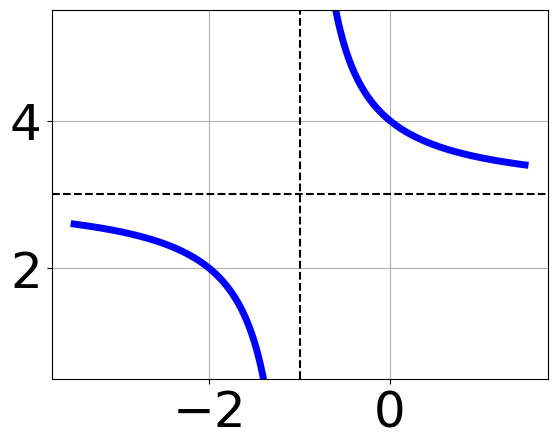
\includegraphics[width=0.3\textwidth]{../Figures/rationalEquationToGraphCopyDC.png}
\end{center}\begin{enumerate}[label=\Alph*.]
\begin{multicols}{2}
\item 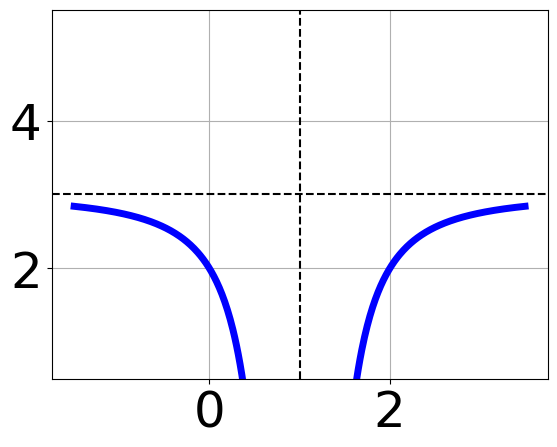
\includegraphics[width = 0.3\textwidth]{../Figures/rationalEquationToGraphCopyAC.png}
\item 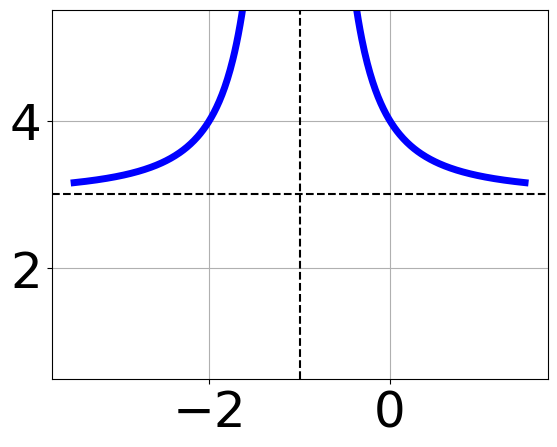
\includegraphics[width = 0.3\textwidth]{../Figures/rationalEquationToGraphCopyBC.png}
\item 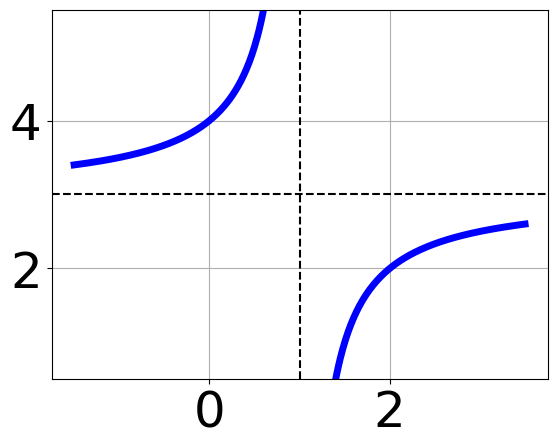
\includegraphics[width = 0.3\textwidth]{../Figures/rationalEquationToGraphCopyCC.png}
\item 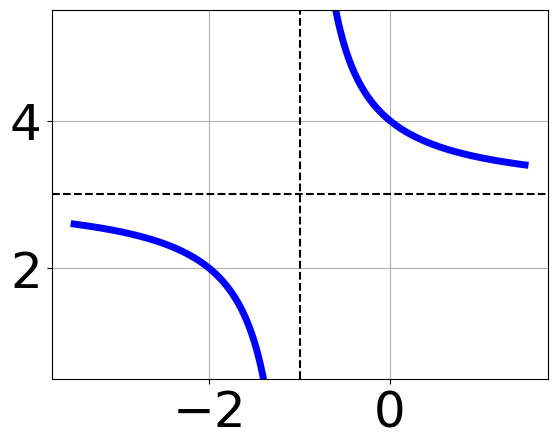
\includegraphics[width = 0.3\textwidth]{../Figures/rationalEquationToGraphCopyDC.png}
\end{multicols}\item None of the above.\end{enumerate}
\textbf{General Comment:} Remember that the general form of a basic rational equation is $ f(x) = \frac{a}{(x-h)^n} + k$, where $a$ is the leading coefficient (and in this case, we assume is either $1$ or $-1$), $n$ is the degree (in this case, either $1$ or $2$), and $(h, k)$ is the intersection of the asymptotes.
}
\litem{
Choose the equation of the function graphed below.

\begin{center}
    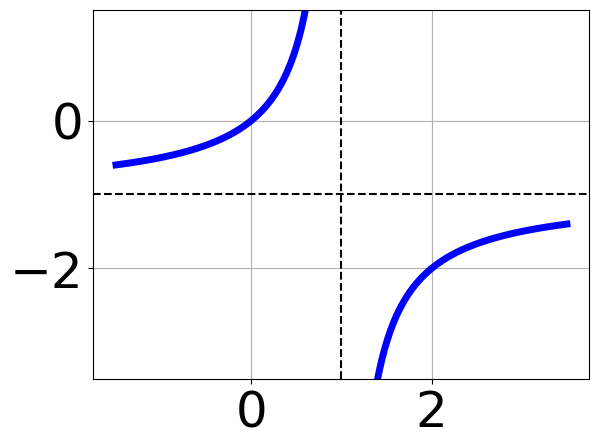
\includegraphics[width=0.5\textwidth]{../Figures/rationalGraphToEquationCopyC.png}
\end{center}


The solution is \( \text{None of the above as it should be } f(x) = \frac{-1}{x - 1} - 1 \), which is option E.\begin{enumerate}[label=\Alph*.]
\item \( f(x) = \frac{1}{x + 1} + 3 \)

Corresponds to using the general form $f(x) = \frac{a}{x+h}+k$, the opposite leading coefficient AND not noticing the $y$-value was wrong.
\item \( f(x) = \frac{-1}{x - 1} + 3 \)

The $y$-value of the equation does not match the graph.
\item \( f(x) = \frac{1}{(x + 1)^2} + 3 \)

Corresponds to thinking the graph was a shifted version of $\frac{1}{x^2}$, using the general form $f(x) = \frac{a}{x+h}+k$, the opposite leading coefficient, AND not noticing the $y$-value was wrong.
\item \( f(x) = \frac{-1}{(x - 1)^2} + 3 \)

Corresponds to thinking the graph was a shifted version of $\frac{1}{x^2}$ not noticing the $y$-value was wrong.
\item \( \text{None of the above} \)

None of the equation options were the correct equation.
\end{enumerate}

\textbf{General Comment:} Remember that the general form of a basic rational equation is $ f(x) = \frac{a}{(x-h)^n} + k$, where $a$ is the leading coefficient (and in this case, we assume is either $1$ or $-1$), $n$ is the degree (in this case, either $1$ or $2$), and $(h, k)$ is the intersection of the asymptotes.
}
\litem{
Choose the graph of the equation below.
\[ f(x) = \frac{1}{(x - 2)^2} + 2 \]The solution is the graph below, which is option D.
\begin{center}
    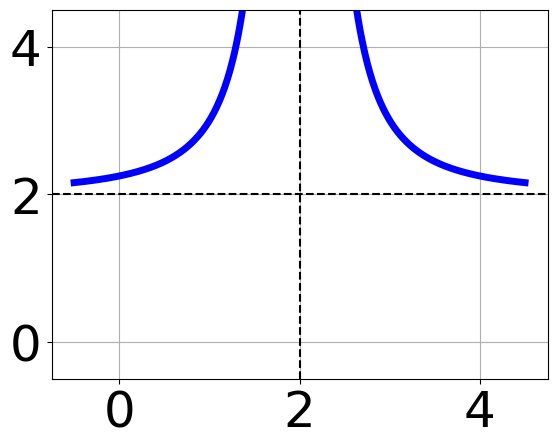
\includegraphics[width=0.3\textwidth]{../Figures/rationalEquationToGraphDC.png}
\end{center}\begin{enumerate}[label=\Alph*.]
\begin{multicols}{2}
\item 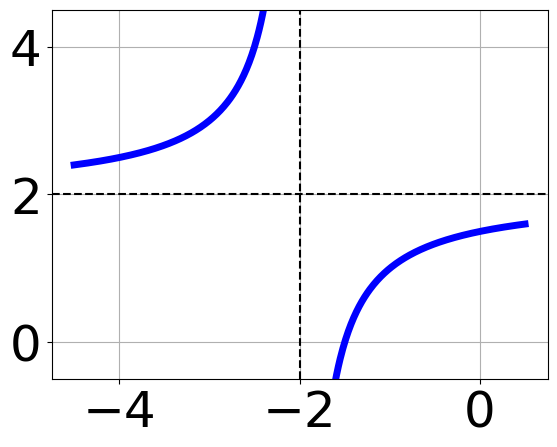
\includegraphics[width = 0.3\textwidth]{../Figures/rationalEquationToGraphAC.png}
\item 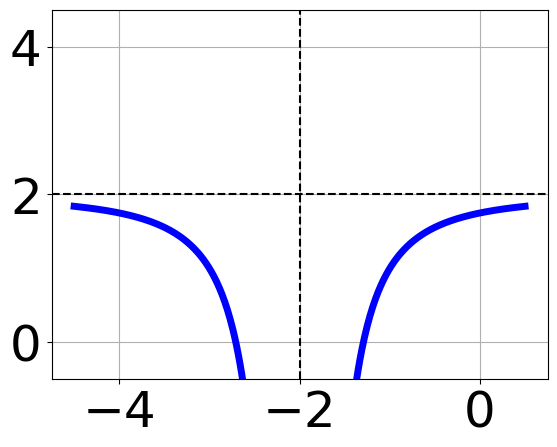
\includegraphics[width = 0.3\textwidth]{../Figures/rationalEquationToGraphBC.png}
\item 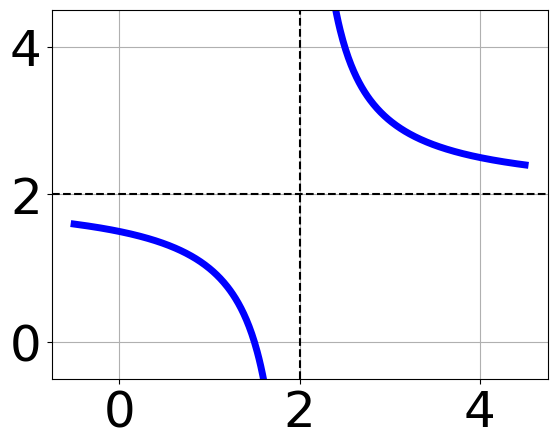
\includegraphics[width = 0.3\textwidth]{../Figures/rationalEquationToGraphCC.png}
\item 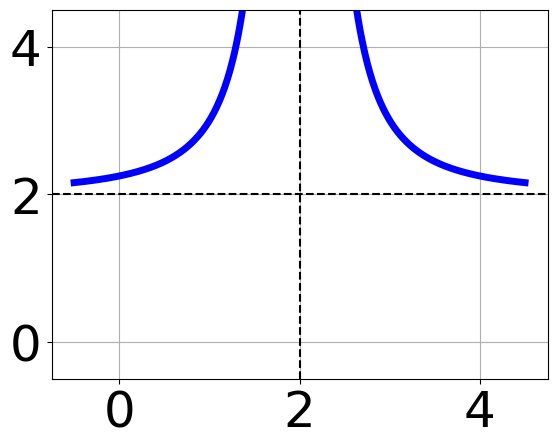
\includegraphics[width = 0.3\textwidth]{../Figures/rationalEquationToGraphDC.png}
\end{multicols}\item None of the above.\end{enumerate}
\textbf{General Comment:} Remember that the general form of a basic rational equation is $ f(x) = \frac{a}{(x-h)^n} + k$, where $a$ is the leading coefficient (and in this case, we assume is either $1$ or $-1$), $n$ is the degree (in this case, either $1$ or $2$), and $(h, k)$ is the intersection of the asymptotes.
}
\litem{
Solve the rational equation below. Then, choose the interval(s) that the solution(s) belongs to.
\[ \frac{88}{44x -22} + 1 = \frac{88}{44x -22} \]The solution is \( \text{all solutions are invalid or lead to complex values in the equation.} \), which is option D.\begin{enumerate}[label=\Alph*.]
\item \( x \in [-1.3,-0.4] \)

$x = -0.500$, which corresponds to not distributing the factor $44x -22$ correctly when trying to eliminate the fraction.
\item \( x_1 \in [-1.3, -0.4] \text{ and } x_2 \in [0.5,1.5] \)

$x = -0.500 \text{ and } x = 0.500$, which corresponds to getting the correct solution and believing there should be a second solution to the equation.
\item \( x \in [0.5,1.5] \)

$x = 0.500$, which corresponds to not checking if this value leads to dividing by 0 in the original equation and thus is not a valid solution.
\item \( \text{All solutions lead to invalid or complex values in the equation.} \)

*$x = 0.500$ leads to dividing by 0 in the original equation and thus is not a valid solution, which is the correct option.
\item \( x_1 \in [0.3, 1.5] \text{ and } x_2 \in [0.5,1.5] \)

$x = 0.500 \text{ and } x = 0.500$, which corresponds to getting the correct solution and believing there should be a second solution to the equation.
\end{enumerate}

\textbf{General Comment:} Distractors are different based on the number of solutions. Remember that after solving, we need to make sure our solution does not make the original equation divide by zero!
}
\litem{
Solve the rational equation below. Then, choose the interval(s) that the solution(s) belongs to.
\[ \frac{-6x}{-7x -7} + \frac{-2x^{2}}{14x^{2} +49 x + 35} = \frac{-3}{-2x -5} \]The solution is \( \text{There are two solutions: } x = 1.067 \text{ and } x = -1.967 \), which is option A.\begin{enumerate}[label=\Alph*.]
\item \( x_1 \in [0.96, 1.29] \text{ and } x_2 \in [-3.59,-1.43] \)

* $x = 1.067 \text{ and } x = -1.967$, which is the correct option.
\item \( \text{All solutions lead to invalid or complex values in the equation.} \)


\item \( x_1 \in [0.96, 1.29] \text{ and } x_2 \in [-1.5,-0.92] \)


\item \( x \in [-3.1,-2.03] \)


\item \( x \in [-2.28,-1.93] \)


\end{enumerate}

\textbf{General Comment:} Distractors are different based on the number of solutions. Remember that after solving, we need to make sure our solution does not make the original equation divide by zero!
}
\litem{
Determine the domain of the function below.
\[ f(x) = \frac{5}{24x^{2} -14 x -20} \]The solution is \( \text{All Real numbers except } x = -0.667 \text{ and } x = 1.250. \), which is option A.\begin{enumerate}[label=\Alph*.]
\item \( \text{All Real numbers except } x = a \text{ and } x = b, \text{ where } a \in [-1.9, -0.1] \text{ and } b \in [0.6, 2.8] \)

All Real numbers except $x = -0.667$ and $x = 1.250$, which is the correct option.
\item \( \text{All Real numbers except } x = a \text{ and } x = b, \text{ where } a \in [-25.1, -23.2] \text{ and } b \in [19.1, 20.6] \)

All Real numbers except $x = -24.000$ and $x = 20.000$, which corresponds to not factoring the denominator correctly.
\item \( \text{All Real numbers except } x = a, \text{ where } a \in [-25.1, -23.2] \)

All Real numbers except $x = -24.000$, which corresponds to removing a distractor value from the denominator.
\item \( \text{All Real numbers except } x = a, \text{ where } a \in [-1.9, -0.1] \)

All Real numbers except $x = -0.667$, which corresponds to removing only 1 value from the denominator.
\item \( \text{All Real numbers.} \)

This corresponds to thinking the denominator has complex roots or that rational functions have a domain of all Real numbers.
\end{enumerate}

\textbf{General Comment:} Recall that dividing by zero is not a real number. Therefore the domain is all real numbers \textbf{except} those that make the denominator 0.
}
\litem{
Solve the rational equation below. Then, choose the interval(s) that the solution(s) belongs to.
\[ \frac{3}{3x -2} + 6 = \frac{-2}{27x -18} \]The solution is \( x = 0.488 \), which is option D.\begin{enumerate}[label=\Alph*.]
\item \( \text{All solutions lead to invalid or complex values in the equation.} \)

This corresponds to thinking $x = 0.488$ leads to dividing by zero in the original equation, which it does not.
\item \( x_1 \in [0.26, 0.47] \text{ and } x_2 \in [-0.51,3.49] \)

$x = 0.389 \text{ and } x = 0.488$, which corresponds to getting the correct solution and believing there should be a second solution to the equation.
\item \( x \in [-0.89,-0.84] \)

$x = -0.846$, which corresponds to not distributing the factor $3x -2$ correctly when trying to eliminate the fraction.
\item \( x \in [0.49,2.49] \)

* $x = 0.488$, which is the correct option.
\item \( x_1 \in [-0.89, -0.84] \text{ and } x_2 \in [-0.51,3.49] \)

$x = -0.846 \text{ and } x = 0.488$, which corresponds to getting the correct solution and believing there should be a second solution to the equation.
\end{enumerate}

\textbf{General Comment:} Distractors are different based on the number of solutions. Remember that after solving, we need to make sure our solution does not make the original equation divide by zero!
}
\litem{
Solve the rational equation below. Then, choose the interval(s) that the solution(s) belongs to.
\[ \frac{-4x}{5x -5} + \frac{-7x^{2}}{-35x^{2} + 35} = \frac{-5}{-7x -7} \]The solution is \( \text{There are two solutions: } x = 0.406 \text{ and } x = -2.930 \), which is option C.\begin{enumerate}[label=\Alph*.]
\item \( x \in [-2.4,-0.1] \)


\item \( \text{All solutions lead to invalid or complex values in the equation.} \)


\item \( x_1 \in [-0.4, 0.7] \text{ and } x_2 \in [-6.93,-0.93] \)

* $x = 0.406 \text{ and } x = -2.930$, which is the correct option.
\item \( x_1 \in [-0.4, 0.7] \text{ and } x_2 \in [0,11] \)


\item \( x \in [-5.1,-1.5] \)


\end{enumerate}

\textbf{General Comment:} Distractors are different based on the number of solutions. Remember that after solving, we need to make sure our solution does not make the original equation divide by zero!
}
\litem{
Choose the equation of the function graphed below.

\begin{center}
    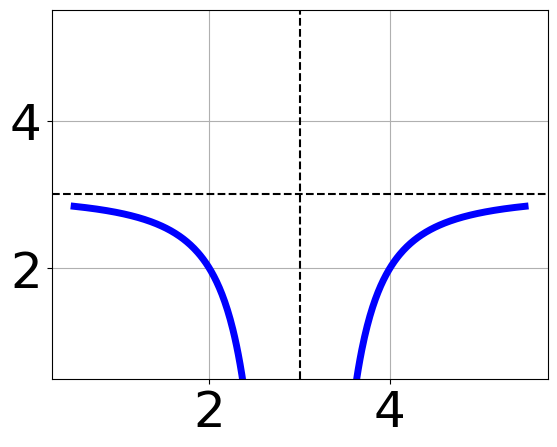
\includegraphics[width=0.5\textwidth]{../Figures/rationalGraphToEquationC.png}
\end{center}


The solution is \( \text{None of the above as it should be } f(x) = \frac{-1}{(x - 3)^2} + 3 \), which is option E.\begin{enumerate}[label=\Alph*.]
\item \( f(x) = \frac{-1}{x + 3} + 1 \)

Corresponds to thinking the graph was a shifted version of $\frac{1}{x}$ AND not noticing the $y$-value was wrong.
\item \( f(x) = \frac{1}{x - 3} + 1 \)

Corresponds to thinking the graph was a shifted version of $\frac{1}{x}$, using the general form $f(x) = \frac{a}{(x-h)^2}+k$, the opposite leading coefficient, AND not noticing the $y$-value was wrong.
\item \( f(x) = \frac{1}{(x - 3)^2} + 1 \)

Corresponds to using the general form $f(x) = \frac{a}{(x-h)^2}+k$, the opposite leading coefficient, AND not noticing the $y$-value was wrong.
\item \( f(x) = \frac{-1}{(x + 3)^2} + 1 \)

The $x$- and $y$-value of the equation does not match the graph.
\item \( \text{None of the above} \)

None of the equation options were the correct equation.
\end{enumerate}

\textbf{General Comment:} Remember that the general form of a basic rational equation is $ f(x) = \frac{a}{(x-h)^n} + k$, where $a$ is the leading coefficient (and in this case, we assume is either $1$ or $-1$), $n$ is the degree (in this case, either $1$ or $2$), and $(h, k)$ is the intersection of the asymptotes.
}
\end{enumerate}

\end{document}